\documentclass[a4paper, 11pt, twoside]{article}

%\usepackage[ngerman]{babel}
\usepackage[english]{babel}
\usepackage[latin1]{inputenc}

\usepackage{graphicx,float}
%\usepackage{pifont}
\usepackage{type1cm}
\usepackage{amssymb, amsthm, amsmath}
\usepackage{listings}
\usepackage{pgf}
\usepackage{url}
\usepackage{hyperref}
\usepackage{rotating}
\usepackage{makeidx}
\makeindex

\setlength{\parindent}{0em}
\setlength{\oddsidemargin}{0.0cm}
\setlength{\evensidemargin}{0.0cm}
\setlength{\textheight}{24.0cm}
\setlength{\topmargin}{-1.0cm}
\setlength{\footskip}{1.5cm}
\setlength{\textwidth}{15.5cm}

\renewcommand*\familydefault{\sfdefault}
\newcommand{\dd}{\mathrm{d}}
\newtheorem{problem}{Problem}[section]
\newtheorem{theorem}{Theorem}[section]
\newtheorem{remark}{Remark}[section]

%%%% Environnement pour modifier localement les marges %%%%
\newenvironment{changemargin}[2]{\begin{list}{}{%
\setlength{\topsep}{0pt}%
\setlength{\leftmargin}{0pt}%
\setlength{\rightmargin}{0pt}%
\setlength{\listparindent}{\parindent}%
\setlength{\itemindent}{\parindent}%
\setlength{\parsep}{0pt plus 1pt}%
\addtolength{\leftmargin}{#1}%
\addtolength{\rightmargin}{#2}%
}\item }{\end{list}}
%%%% fin  %%%%


\begin{document}

%\documentclass[a4paper]{article}

%\usepackage{pgf}
%\usepackage{graphicx}
%\usepackage{pifont}
%\usepackage{type1cm}

\setlength{\textwidth}{14cm}
\setlength{\oddsidemargin}{1cm}

%\begin{document}

\pagestyle{empty}

%%%%%%%%%%%%%%%%%%%%%%%%%%%%%%%%%%%%%%%%
%%%%%%%%%%%%%%%%%%%%%%%%%%%%%%%%%%%%%%%%
%%%%%%%%%%%%%%%%%%%%%%%%%%%%%%%%%%%%%%%%

\newcount \Z
\Z=20

%%% logos %%%

%%% NUMHPC %%%
\newlength{\numhpclogox}
\setlength{\numhpclogox}{\paperwidth} % 20/210ths of the paperwidth
\divide\numhpclogox by 210
\multiply\numhpclogox by 100

\newlength{\numhpclogoy}
\setlength{\numhpclogoy}{\paperheight} % 270/297ths of the paperwidth
\divide \numhpclogoy by 297
\multiply \numhpclogoy by -235

\newlength{\numhpclogoheight}
\setlength{\numhpclogoheight}{\paperheight} % 270/297ths of the paperwidth
\divide\numhpclogoheight by 297
\multiply\numhpclogoheight by 20

%%% KIT %%%
\newlength{\kitlogox}
\setlength{\kitlogox}{\paperwidth} % 20/210ths of the paperwidth
\divide\kitlogox by 210
\multiply\kitlogox by 0

\newlength{\kitlogoy}
\setlength{\kitlogoy}{\paperheight} % 270/297ths of the paperwidth
\divide \kitlogoy by 297
\multiply \kitlogoy by -230

\newlength{\kitlogoheight}
\setlength{\kitlogoheight}{\paperheight} % 270/297ths of the paperwidth
\divide\kitlogoheight by 297
\multiply\kitlogoheight by 15


%%% EMCL %%%
\newlength{\emcllogox}
\setlength{\emcllogox}{\paperwidth} % 20/210ths of the paperwidth
\divide\emcllogox by 210
\multiply\emcllogox by 28

\newlength{\emcllogoy}
\setlength{\emcllogoy}{\paperheight} % 270/297ths of the paperwidth
\divide \emcllogoy by 297
\multiply \emcllogoy by -160

\newlength{\emcllogoheight}
\setlength{\emcllogoheight}{\paperheight} % 270/297ths of the paperwidth
\divide\emcllogoheight by 297
\multiply\emcllogoheight by 20

%%% HIFLOW %%%
\newlength{\hiflowlogox}
\setlength{\hiflowlogox}{\paperwidth} % 20/210ths of the paperwidth
\divide\hiflowlogox by 210
\multiply\hiflowlogox by 28

\newlength{\hiflowlogoy}
\setlength{\hiflowlogoy}{\paperheight} % 270/297ths of the paperwidth
\divide \hiflowlogoy by 297
\multiply \hiflowlogoy by -160

\newlength{\hiflowlogoheight}
\setlength{\hiflowlogoheight}{\paperheight} % 270/297ths of the paperwidth
\divide\hiflowlogoheight by 297
\multiply\hiflowlogoheight by 33

%%%%%%%%%%%%%%%%%%%%%%%%%%%%%%%%%%%%%%%%
%%%%%%%%%%%%%%%%%%%%%%%%%%%%%%%%%%%%%%%%
%%%%%%%%%%%%%%%%%%%%%%%%%%%%%%%%%%%%%%%%

%%% NUMHPC %%%
%%\pgftext[bottom, left, at={\pgfpointadd{\pgfpoint{0pt}{0pt}}{\pgfpoint{\numhpclogox}{\numhpclogoy}}}]{\includegraphics[totalheight=\numhpclogoheight]{numhpc}}

%%% KIT %%%
%%\pgftext[bottom, left, at={\pgfpointadd{\pgfpoint{0pt}{0pt}}{\pgfpoint{\kitlogox}{\kitlogoy}}}]{\includegraphics[totalheight=\kitlogoheight]{kitlogo}}

%%% EMCL %%%
\pgftext[bottom, left, at={\pgfpointadd{\pgfpoint{0pt}{0pt}}{\pgfpoint{\hiflowlogox}{\hiflowlogoy}}}]{
\includegraphics[totalheight=\hiflowlogoheight]{HF3_color}}

%%% horizontal lines %%%
\pgfline{\pgfxy(-1pt,0.1pt)}{\pgfxy(15pt,0.1pt)}
\pgfline{\pgfxy(-1pt,-21.4pt)}{\pgfxy(15pt,-21.4pt)}
%%\pgfline{\pgfxy(-1pt,-22.4pt)}{\pgfxy(15pt,-22.4pt)}

%%% EMCL text %%%
\pgftext[bottom, left, at={\pgfpointadd{\pgfpoint{0pt}{0pt}}{\pgfpoint{0cm}{1cm}}}]{{\LARGE{{\bf Tutorial}}}}


%%% EMCL web %%%
\pgftext[bottom, left, at={\pgfpointadd{\pgfpoint{0pt}{0pt}}{\pgfpoint{10.5cm}{-21.7cm}}}]{{\fontsize{13}{10}\selectfont{} http://www.hiflow3.org/}}

\hspace{2cm}
\begin{picture}(0,0)(-250,-25)

\includegraphics[scale=.22]{emcl.pdf} 
\end{picture}

%%% author %%%
\pgftext[bottom, left, at={\pgfpointadd{\pgfpoint{0pt}{0pt}}{\pgfpoint{0cm}{-4cm}}}]{{
\begin{parbox}{13cm}{
\begin{center}\fontsize{12}{30}\selectfont{} T. Delerue, E. Ketelaer, M. Schick
\end{center}}
\end{parbox}}}

%%% title %%%
\pgftext[bottom, left, at={\pgfpointadd{\pgfpoint{0pt}{0pt}}{\pgfpoint{0cm}{-7.5cm}}}]{{
\begin{parbox}{13cm}{
%%\begin{center}\fontsize{18}{30}\selectfont{} \bf Applying HiFlow$^3$ for solving the
\begin{center}\fontsize{22}{30}\selectfont{} \bf Applying an Inexact Newton Method in Hiflow$^3$
\end{center}}
\end{parbox}}}

%%% date %%%
\pgftext[bottom, left, at={\pgfpointadd{\pgfpoint{0pt}{0pt}}{\pgfpoint{0cm}{-16.4cm}}}]{{
\begin{parbox}{13cm}{
\begin{center}\fontsize{12}{24}\selectfont{} 
\vspace{5cm}
\textit{modified on \today}\\ 
\vspace{6.5cm}
\hspace{6cm}\textit{Version 1.3}
\end{center}}
\end{parbox}}}

%fhfh \hfill sjdh

%\end{document}


\tableofcontents

\newpage
\pagestyle{plain}
\framebox[15.5cm]{\parbox[c][2.3cm]{14.5cm}{
{\fontsize{19}{19}\selectfont{} \bf{Applying an Inexact Newton Method in HiFlow$^3$}
}}}
\vspace{0.5cm}

\section{Introduction}
HiFlow$^3$ is a multi-purpose finite element software providing powerful tools for efficient and accurate solution of a wide range of problems modeled by partial differential equations (PDEs). Based on object-oriented concepts and the full capabilities of C++ the HiFlow$^3$ project follows a modular and generic approach for building efficient parallel numerical solvers. It provides highly capable modules dealing with the mesh setup, finite element spaces, degrees of freedom, linear algebra routines, numerical solvers, and output data for visualization. Parallelism - as the basis for high performance simulations on modern computing systems - is introduced on two levels: coarse-grained parallelism by means of distributed grids and distributed data structures, and fine-grained parallelism by means of platform-optimized linear algebra back-ends.

\subsection{How to use the tutorial?}
You find the example codes \verb+newton_tutorial.cc+ and \verb+newton_tutorial.h+ and a parameter file \verb+newton_tutorial.xml+ for a numerical example in the folder \verb'/hiflow/examples/newton'. The geometry data (*.inp, *.vtu) is stored in the folder \verb'/hiflow/examples/data'.

\subsubsection{Using HiFlow$^3$ as a Developer}\label{sectiondeveloper}
First build and compile HiFlow$^3$. Go to the directory \verb'/build/example/newton', where the binary \textbf{newton\_tutorial} is stored. Type \textbf{./newton\_tutorial}, to execute the program in sequential mode. To execute in parallel mode \index{program!executing in parallel} with four processes, type \textbf{mpirun -np 4 ./newton\_tutorial}. In both cases, you need to make sure that the default parameterfile newton\_tutorial.xml is stored in the same directory as the binary, and that the geometry data specified in the parameter file is stored in \verb'/hiflow/examples/data'. Alternatively, you can specify the path of your own xml-file with the name of your xml-file (first) and the path of your geometry data (second) in the comment line, i.e. \textbf{./newton\_tutorial} \verb'/"path_to_parameterfile"/"name_of_parameterfile".xml' \verb'/"path_to_geometry_data"/'.

\section{Mathematical Setup}


\subsection{Problem} \label{problem}
In this tutorial we are trying to observe the effect of inexact Newton methods on the calculation time of a fluid dynamics problem. For this purpose two particular methods developed by Eisenstat and Walker~\cite{EW}, which are already implemented in Hiflow$^3$~\cite{hiflow3:nonlinear} were used. The problem consists of solving the incompressible Navier-Stokes equations in a two-dimensional channel around a rectangular obstacle(see figure ~\ref{channel}). For this purpose we applied the same model as in the Hiflow$^3$ tutorial \emph{Boundary Value Problem for Incompressible Navier-Stokes Equation}, thus for complete informations regarding the mathematical and geometry setup we refer to ~\cite{Tut}. We first give a brief overview of the theory behind exact and inexact Newton methods, then we mention the source code of the tutorial, and we finish by presenting the obtained results.

\setlength{\unitlength}{1cm}
\begin{figure}[!h]
	\centering
		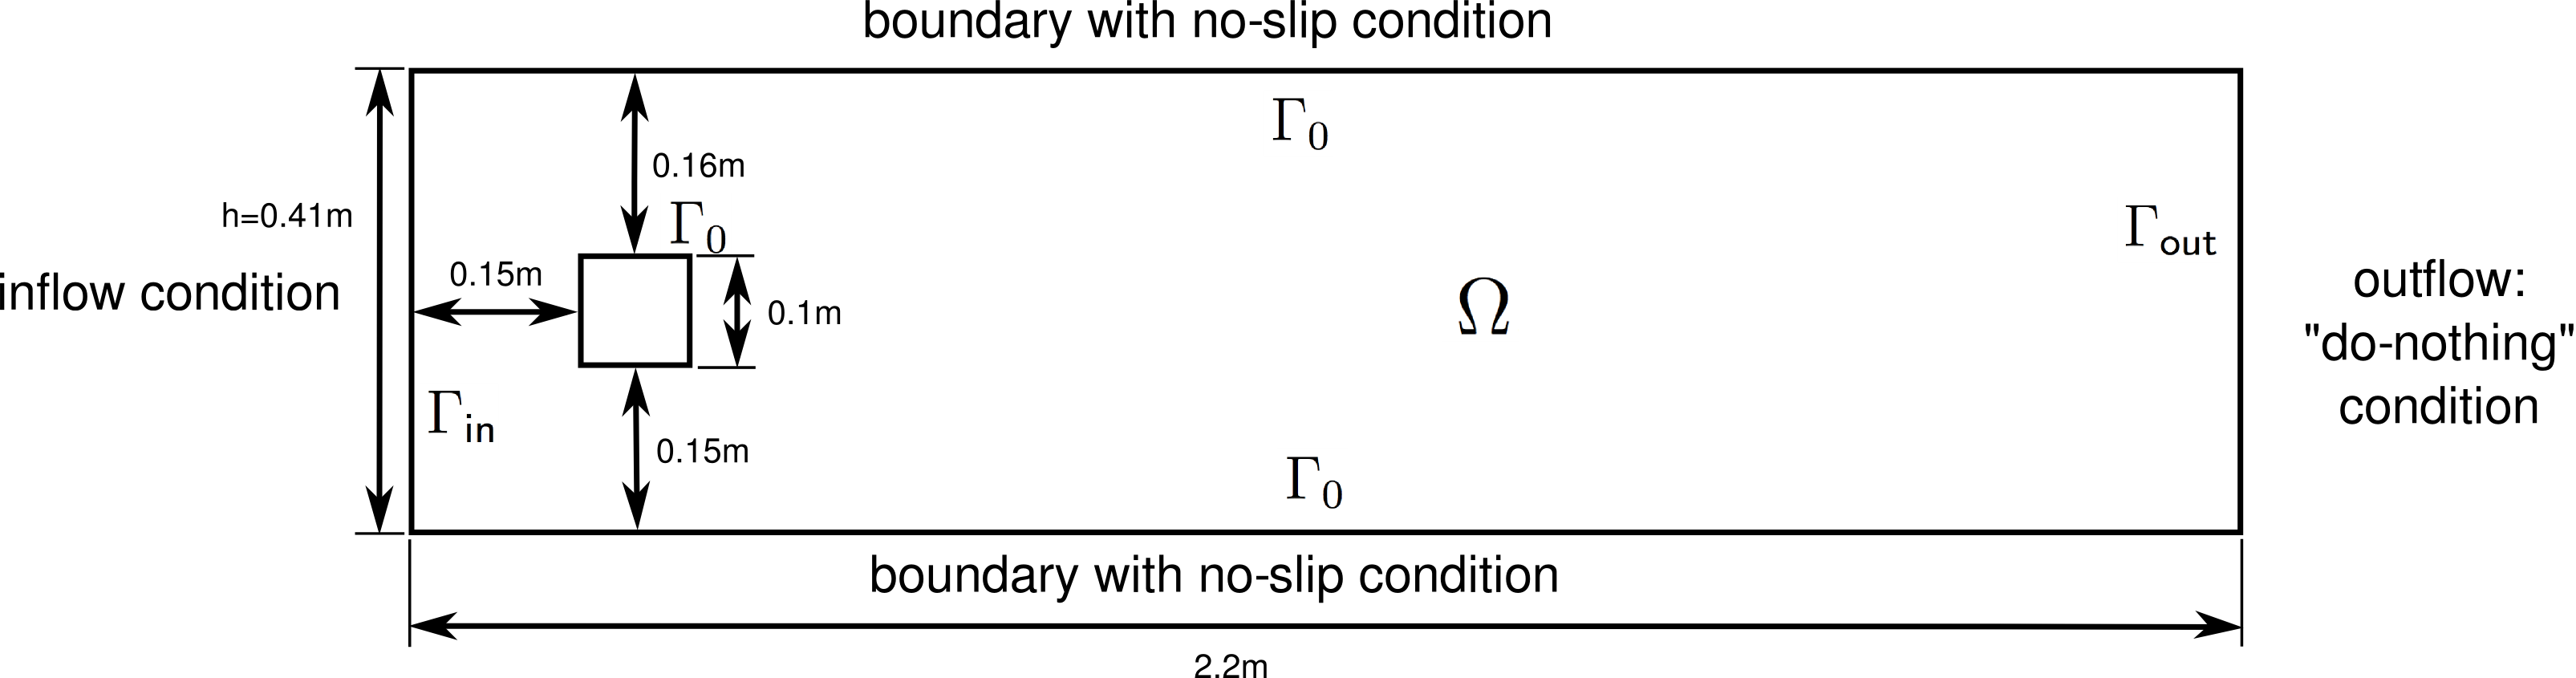
\includegraphics[width=1.1\textwidth]{fig/Zeichnung_Kanal_en.png}
		\begin{picture}(1,1)(-1.25,-1.2)
		\put(-8.2,1.6){\footnotesize{$u(x_1, x_2) =$}}
		\put(-8.2,1.1){\footnotesize{$g(x_1, x_2)$}}
		\put(1.1,3.7){\footnotesize{$u(x_1, x_2) = 0$}}
		\put(1.1,0.35){\footnotesize{$u(x_1, x_2) = 0$}}
		\end{picture}
\vspace{-0.75cm}
\caption{Flow channel in 2D with an obstacle.}
\label{channel}
\end{figure}



\subsection{Exact and Inexact Newton Methods} \label{theorie}
The exact Newton method originally solves a nonlinear problem \index{nonlinear!problem} equation~\cite{newton:method} of the form 
\begin{equation} \label{newton1}
F(x)=0,
\end{equation}
where $F$ is a nonlinear operator $F: D \subset X \to Y$ and $X$, $Y$ Banach spaces endowed with norms $ \Vert \cdot \Vert_X$, $ \Vert \cdot \Vert_Y$. In addition, $F$ needs to be at least once continuously differentiable, and a starting guess $x^0$ for the solution of (\ref{newton1}) is necessary. Linearization of $F$ at $x^0$, by means of Taylor's expansion of first order, leads to the linear equation $F'(x^0) \Delta x^0 + F(x^0)=0$. The solution $\Delta x^0$ is then added to the starting guess, leading to a new solution vector $x^1$. A linearization of $F$, this time at $x^1$, leads to a new linear equation which in turn provides a new increment $\Delta x^1$. Repetition of these steps leads therefore to an iteration rule which approximates (\ref{newton1}):
\begin{equation} \label{newton2}
F'(x^k) \Delta x^k + F(x^k)=0, \qquad
x^{k+1}=x^k+\Delta x^k, \qquad k=0,1,...
\end{equation}
Thus, the nonlinear problem (\ref{newton1}) turns into a sequence of linear problems. This is called Newton's method for general nonlinear problems. In our situation iteration (\ref{newton2}) (nonlinear solver) is pursued until the residual \index{Residual} $F(x^k)$, evaluated at the so-called Newton step $k$ \index{Newton step}, respects some conditions set prior to calculation, that is, tolerances on the iterative residual norm $\Vert F(x^k)\Vert_Y$ and on the iterative ratio $\frac{\Vert F(x^k) \Vert_Y}{\Vert F(x^{k-1}) \Vert_Y}$ \index{Relative tolerance}. Now, at each Newton step $k$ a linear solver \index{Linear!solver} is launched in Hiflow$^3$ in order to determine the $k$-th increment $\Delta x^k$. Check of convergence takes place here at the linear residual \index{Linear!residual} norm $\Vert F'(x^k) \Delta x^k + F(x^k) \Vert_Y$ at the Newton step $k$, as well as at the following ratio:
\begin{equation}\label{ratio}
\frac{\Vert F'(x^k) \Delta x^k + F(x^k)\Vert_Y}{\Vert F(x^k) \Vert_Y}
\end{equation}
In an \textbf{exact Newton method} \index{Newton method!exact} strong absolute and relative tolerances are set, as can be seen in table ~\ref{CC}. In comparison \textbf{inexact newton methods} \index{Newton method!inexact} aim at loosening up the tolerance on the above mentioned ratio in order to gain calculation time without loosing too much accuracy. In fact at each Newton step $k$ a so called forcing term \index{Forcing!term} $\eta_k \in \lbrack 0, 1)$ is calculated and the stopping point is reached as soon as the linear residual respects the condition
\begin{equation}
\frac{\Vert F'(x^k) \Delta x^k + F(x^k) \Vert_Y}{\Vert F(x^k) \Vert_Y} \leq \eta_k .
\end{equation}
The tolerance on the linear residual norm is left unchanged. Hence we observe that the main difference between both approaches lies in the choice of the upper bound of the ratio~(\ref{ratio}), which remains constant in an exact Newton method but varies in an inexact Newton method at each Newton step $k$.

As mentioned in section ~\ref{problem} two methods \cite{EW} were applied in this tutorial. In these methods the forcing term $\eta_k$ at each Newton step $k$ is calculated as follows: \\
Choice 1 (\textbf{Forcing strategy 1} \index{Forcing!strategy})~\label{choice1}
\begin{equation}
\eta_k = \frac{\mid \Vert F(x^k) \Vert_Y - \Vert F'(x^{k-1}) \Delta x^{k-1} + F(x^{k-1}) \Vert_Y \mid}{\Vert F(x^{k-1}) \Vert_Y},
\end{equation}
Choice 2 (\textbf{Forcing strategy 2})~\label{choice2}
\begin{equation} \label{choice2}
\eta_k = \gamma \bigg( \frac{\Vert F(x^k) \Vert_Y}{\Vert F(x^{k-1}) \Vert_Y} \bigg)^{\alpha},
\end{equation}
where a start value $\eta_0 \in \lbrack 0, 1)$ as well as the parameters $\gamma \in \lbrack 0, 1\rbrack $, $\alpha \in (1, 2\rbrack$ are given. For a thorough motivation of the choice of these two particular forcing terms and the related parameters see ~\cite{EW}. \\ 
These two inexact Newton methods as well as the exact Newton method are contained in Hiflow$^3$~\cite{hiflow3:nonlinear}. In the following we present how to apply them.


\section{The Commented Program}
\subsection{Preliminaries}
The Newton tutorial needs following two input files:
\begin{itemize}
\item A parameter file: The parameter file is an xml-file, which contains all parameters needed to execute the program. It is read in by the program. Parameters for example defining the termination condition of the nonlinear and linear solver are listed as well as parameters needed for the linear algebra. It is not necessary to recompile the program, when parameters in the xml-file are changed. By default the Newton tutorial reads in the parameter file \verb+newton_tutorial.xml+, see section \ref{sectionparameter file}, which contains the parameters of the two-dimensional numerical example. This file is stored in \verb'/hiflow/examples/newton/'. 
\item Geometry data\index{geometry data}: The file containing the geometry is specified in the parameter file. For the numerical results in two dimensions we choose \textbf{dfg2d\_rect.inp}. You can find different meshes in the folder \verb'/hiflow/examples/data' .
\end{itemize}

HiFlow$^3$ does not generate meshes for the domain $\Omega$. Meshes in *.inp and *.vtu format can be read in. There is a function in \verb'/build/utils/' called 'inp2vtu' which converts *.inp format to *.vtu format. Type \textbf{/build/utils/inp2vtu 2 dfg2d\_rect.inp} to convert \verb+dfg2d_rect.inp+ to \verb+dfg2d_rect.vtu+. Additionally a file \verb+dfg2d_rect_bdy.vtu+ is created which shows the body of the domain.\\
It is possible to extend the reader for other formats.
Furthermore it is possible to generate other geometries by using external programs (Mesh generators) or by hand. 
Both formats provide the possibility to mark cell or facets by material numbers.\\ 

To distinguish different boundary conditions, material numbers are set on the boundary different. You can find different material numbers for some given geometry files in table (\ref{materialnumbers}).
\begin{table}[htb]
  \begin{tabular}{|l|l|l|l|l|l|l|l|}
  \hline
  File & \multicolumn{7}{|l|}{Material numbers} \\
  \hline
  & Inflow & Outflow & Top & Bottom & Obstacle & Front & Back \\
  \hline
  dfg2d\_rect.inp & 15 & 16 & 13 & 13 & 14 & - & - \\
  \hline
  channel\_2d\_uniform.inp & 10 & 12 & 13 & 11 & none & - & - \\
  \hline
  dfg\_bench3d\_cyl.inp & 10 & 12 & 11 & 11 & 13 & 11 & 11 \\
  \hline
  dfg\_bench3d\_rect2.inp & 10 & 12 & 11 & 11 & 13 & 30 & 20 \\
  \hline
  channel\_bench1.inp & 10 & 12 & 13 & 11 & 2/1(up/down) & 30 & 20 \\
  \hline
  \end{tabular}
\caption{Material numbers\index{material numbers} for different geometry files}
\label{materialnumbers}
\end{table}
The parameter file defines the meaning of the material number:
In the parameter file you find the boundary parameters InflowMaterial and OutflowMaterial. 
In this case the variable InflowMaterial is set to 15 and the variable OutflowMaterial to 16.\\

The Newton tutorial emerges from an already existing program in Hiflow$^3$, \verb+channel_benchmark+, whose source code is contained in  \verb+hiflow//examples/benchmarks/channel_benchmark/+. The source code was slightly modified in order to make use of the different parts contained in Hiflow$^3$ regarding the inexact Newton methods described in~\ref{theorie}, that is, the classes \verb+ForcingStrategy<LAD>+, its derivative \verb+EWForcing<LAD>+, and \verb+NonlinearSolverParameter+~\cite{hiflow3:nonlinear}.

\subsection{Parameter File} \label{sectionparameter file}
The parameter file normally required by the program \verb+channel_benchmark+ was modified in order to consider the different test parameters  concerning the forcing strategy.

\begin{lstlisting}[language=C++, basicstyle={\footnotesize, \ttfamily}, keywordstyle=\color{blue}, numbers=none, tabsize=4]    
<Param>
  <OutputPrefix>NewtonTutorial</OutputPrefix>
  <Mesh>
    <Filename>dfg2d_rect.inp</Filename>
    <InitialRefLevel>0</InitialRefLevel>
  </Mesh>
  <LinearAlgebra>
    <Platform>CPU</Platform>
    <Implementation>Naive</Implementation>
    <MatrixFormat>CSR</MatrixFormat>
  </LinearAlgebra>
  <FlowModel>
    <Density>1.0</Density>
    <Viscosity>1.0e-3</Viscosity>
    <InflowSpeed>0.5</InflowSpeed>
    <InflowHeight>0.41</InflowHeight>
    <InflowWidth>0.41</InflowWidth>
  </FlowModel>
  <QuadratureOrder>6</QuadratureOrder>
  <FiniteElements>
    <VelocityDegree>2</VelocityDegree>
    <PressureDegree>1</PressureDegree>
  </FiniteElements>
  <Boundary>
    <InflowMaterial>15</InflowMaterial>
    <OutflowMaterial>16</OutflowMaterial>
    <CylinderMaterial>14</CylinderMaterial>
  </Boundary>
  <NonlinearSolver>    
    <MaximumIterations>20</MaximumIterations>
    <AbsoluteTolerance>1.e-15</AbsoluteTolerance>
    <RelativeTolerance>1.e-6</RelativeTolerance>
    <DivergenceLimit>1.e6</DivergenceLimit>    
    <ForcingStrategy>None</ForcingStrategy>
    <InitialValueForcingTerm>0.5</InitialValueForcingTerm>
    <MaxValueForcingTerm>0.9</MaxValueForcingTerm>
    <GammaParameterEW2>1.0</GammaParameterEW2>
    <AlphaParameterEW2>1.618033989</AlphaParameterEW2>
  </NonlinearSolver>
  <LinearSolver>
    <MaximumIterations>100000</MaximumIterations>
    <AbsoluteTolerance>1.e-15</AbsoluteTolerance>
    <RelativeTolerance>1.e-6</RelativeTolerance>
    <DivergenceLimit>1.e6</DivergenceLimit>
    <BasisSize>500</BasisSize>
    <Preconditioning>1</Preconditioning>
  </LinearSolver>
  <ILUPP>
    <PreprocessingType>0</PreprocessingType>
    <PreconditionerNumber>11</PreconditionerNumber>
    <MaxMultilevels>20</MaxMultilevels>
    <MemFactor>0.8</MemFactor>
    <PivotThreshold>2.75</PivotThreshold>
    <MinPivot>0.05</MinPivot>
  </ILUPP>
  <Backup>
    <Restore>0</Restore>
    <LastTimeStep>160</LastTimeStep>
    <Filename>backup.h5</Filename>
  </Backup>
</Param>
\end{lstlisting}

In the field \verb+<ForcingStrategy>  </ForcingStrategy>+ we can choose between the following options: \verb+None+, \verb+EisenstatWalker1+ or \verb+EisenstatWalker2+. For more details regarding the numerical values of the linear and nonlinear solver parameters, see section \ref{results:1}.

\subsection{Main Function}
The main function starts the simulation of the Newton tutorial \verb+newton_tutorial.cc+.
\begin{lstlisting}[language=C++, basicstyle={\footnotesize, \ttfamily}, keywordstyle=\color{blue}, numbers=none, tabsize=4]    
int main ( int argc, char** argv )
{
    MPI_Init ( &argc, &argv );

    std::string param_filename ( PARAM_FILENAME );
    if ( argc > 1 )
    {
        param_filename = std::string ( argv[1] );
    }

    try
    {
        NewtonTutorial app ( param_filename );
        app.run ( );
    }
    catch ( const std::exception& e )
    {
        std::cerr << "\nProgram ended with uncaught exception.\n";
        std::cerr << e.what ( ) << "\n";
        return -1;
    }
    MPI_Finalize ( );

    return 0;
}
\end{lstlisting}

\subsection{Member Functions}
Following member functions are components of the Newton tutorial:
\begin{itemize}
\item run()
\item read\_mesh()
\item prepare()
\item prepare\_bc()
\item visualize()
\item EvalFunc(const LAD::VectorType\& in, LAD::VectorType* out)
\item compute\_residual(const LAD::VectorType\& in, LAD::VectorType* out)
\item compute\_stationary\_residual(const LAD::VectorType\& in, LAD::VectorType* out)
\item EvalGrad(const LAD::VectorType\& in, LAD::MatrixType* out)
\item compute\_jacobian(const LAD::VectorType\& in, LAD::MatrixType* out)
\item compute\_stationary\_matrix(const LAD::VectorType\& in, LAD::MatrixType* out)
\item setup\_linear\_algebra()
\end{itemize}

With the exception of \verb+run()+ and \verb+prepare()+, all member functions can be found in the Navier-Stokes Equation tutorial~\cite{Tut}. \verb+run()+ and \verb+prepare()+ are actually also similar to the ones contained in other Hiflow$^3$ tutorials, however they include here code parts regarding the inexact Newton method. 

\subsubsection{prepare()}
In Hiflow$^3$, if a nonlinear problem is to be solved using the Newton method, the class \verb+Newton<LAD>+ is used. The corresponding instance object in the Newton Tutorial is:
\begin{lstlisting}[language=C++, basicstyle={\footnotesize, \ttfamily}, keywordstyle=\color{blue}, numbers=none, tabsize=4]    
	// nonlinear solver
    Newton<LAD> newton_;
\end{lstlisting}
Within this class further instance variables are present and allow the user to switch between the exact and inexact Newton methods, in particular the instance objects \verb+ForcingStratObject\+ of type \verb+ForcingStrategy<LAD>+, and \verb+ForcingStrategy\+ of type \verb+NonlinearSolverParameter+. 
As these are private variables of the class \verb+Newton<LAD>+, we only have access to them by means of the public instance function \verb+SetForcingStrategy+. So if we wish to use an inexact Newton method, we must make use of this function. It takes as parameter an object also of type \verb+ForcingStrategy<LAD>+, which should already have been initialized according to the wished forcing strategy indicated in the parameter file. The function will then initialize the private objects mentionned above by giving \verb+ForcingStratObject\+ the adress of the parameter object, and by setting \verb+ForcingStrategy\+ to the value \verb+NewtonForcingStrategyOwn+. Concretely these steps take place in the member function \verb+prepare()+ as follows.
\begin{itemize}
\item Initialisation of the nonlinear solver:
\begin{lstlisting}[language=C++, basicstyle={\footnotesize, \ttfamily}, keywordstyle=\color{blue}, numbers=none, tabsize=4]
    // get nonlinear solver parameters from parameter file
    nls_max_iter = 
      params_["NonlinearSolver"]["MaximumIterations"].get<int>();
    nls_abs_tol = 
      params_["NonlinearSolver"]["AbsoluteTolerance"].get<double>();
    nls_rel_tol = 
      params_["NonlinearSolver"]["RelativeTolerance"].get<double>();
    nls_div_tol = 
      params_["NonlinearSolver"]["DivergenceLimit"].get<double>();
    
    // setup nonlinear solver
    newton_.InitParameter(&res_, &matrix_);
    newton_.InitParameter(Newton<LAD>::NewtonInitialSolutionOwn);
    newton_.InitControl(nls_max_iter, nls_abs_tol, 
    					nls_rel_tol, nls_div_tol);
    newton_.SetOperator(*this);
    newton_.SetLinearSolver(gmres_);
\end{lstlisting}
\item Initialisation of \verb+ForcingStratObject\+
\begin{lstlisting}[language=C++, basicstyle={\footnotesize, \ttfamily}, keywordstyle=\color{blue}, numbers=none, tabsize=4]
   // get forcing strategy parameters from parameter file
    forcing_strategy_ = 
      params_["NonlinearSolver"]["ForcingStrategy"].get<std::string>();
    eta_initial = 
      params_["NonlinearSolver"]["InitialValueForcingTerm"].get<double>();
    eta_max = 
      params_["NonlinearSolver"]["MaxValueForcingTerm"].get<double>();
    gamma_EW2 = 
      params_["NonlinearSolver"]["GammaParameterEW2"].get<double>();
    alpha_EW2 = 
      params_["NonlinearSolver"]["AlphaParameterEW2"].get<double>();
    
// setup forcing strategy object ForcingStratObject 
// within the nonlinear solver
    if (forcing_strategy_ == "EisenstatWalker1") {
    	EWForcing<LAD>* EW_Forcing = new EWForcing<LAD>(eta_initial, 
    	                                                eta_max, 1);
    	newton_.SetForcingStrategy(*EW_Forcing);
    	
    } else if (forcing_strategy_ == "EisenstatWalker2") {
    	EWForcing<LAD>* EW_Forcing = 
    	new EWForcing<LAD>(eta_initial, eta_max, 2, 
    					   gamma_EW2, alpha_EW2);
    	newton_.SetForcingStrategy(*EW_Forcing);
    }
\end{lstlisting}

\end{itemize}

We see that if a forcing strategy is desired, an object of type \verb+EWForcing<LAD>+, a subclass of \verb+ForcingStrategy<LAD>+, has to be created first with the appropriate parameters, and then transfered to the nonlinear solver \verb+newton_+ of type \verb+Newton<LAD>+ via the function \verb+SetForcingStrategy+ as explained above. On the other hand if we wish to use the exact Newton method, we simply need to type \verb+None+ in the field \verb+<ForcingStrategy>  </ForcingStrategy>+ of the parameter file.

\subsubsection{run()} \label{run}
The instance function \verb+run()+ initialises the problem, and calls in particular the instance function \verb+Solve()+, contained in the nonlinear solver object \verb+newton_+, to solve the stationary flow problem described in~\ref{problem}. It is defined in the class NewtonTutorial. We indicate here only the relevant part of this function, the entire version of it can be found in the folder \verb+/hiflow/examples/newton+.
\begin{lstlisting}[language=C++, basicstyle={\footnotesize, \ttfamily}, keywordstyle=\color{blue}, numbers=none, tabsize=4]

    virtual void run ( ) 
    {
        simul_name_ = params_["OutputPrefix"].get<std::string>( );

        MPI_Comm_rank ( comm_, &rank_ );
        MPI_Comm_size ( comm_, &num_partitions_ );

        [...]

        // Setup timing report
        TimingScope::set_report ( &time_report_ );

        {
            TimingScope tscope ( "Setup" );
            setup_linear_algebra ( );
            read_mesh ( );
            prepare ( );
        }

        [...]

         // Measurement of the global calculation time
        Timer timer;

        newton_.Solve ( &sol_ );
        
        [...]    

        timer.stop ( );

        [...]    

        visualize ( );

        [...]    
    }

\end{lstlisting}

The time measured by the object \verb+timer+ is the value used by the nonlinear solver to make all calculations and is therefore of great interest here, as it is mainly influenced by the choice of the forcing strategy in the parameter file. \\ \\
For more informations regarding the class \verb+Newton<LAD>+, where a nonlinear problem is solved using either the exact or an inexact Newton method as explained in~\ref{theorie}, please see the corresponding program code \verb+newton.cc+ contained in Hiflow$^3$~\cite{hiflow3:nonlinear}.


\section{Numerical Tests} \label{results:1}
\subsection{Test Parameters}
For comparison we launched the tests using both the exact Newton method and the forcing strategies described in section \ref{theorie}. As for the exact Newton method, the used parameters regarding the convergence conditions of the linear solver are detailled in table \ref{CC}.

\begin{table}[h] 

\centering
\begin{tabular}{l|r}
Absolute Tolerance & 1.0E-015 \\
Relative Tolerance & 1.0E-006 \\
Divergence Limit & 1.0E006
\end{tabular} 

\caption{Convergence Conditions of the Linear Solver} \label{CC}

\end{table} 

For both inexact Newton methods only the relative tolerance differs from these values, see~\ref{theorie}. Consequently, the following parameters need to be entered: for both forcing strategies the initial value of the forcing term, viz. $\eta_0$, was set to $0.5$, whereas the maximal value of $\eta_k$ allowed was set to $0.9$ in both cases. In addition, for the second forcing strategy the values of the parameters $\gamma$ and $\alpha$ (see Forcing strategy 2, \ref{choice2}), which were successively tested, are presented in table \ref{FS2}.

\begin{table}[h] 

\centering
\begin{tabular}{rcc|c|c|c}
$\gamma$ && 0.8 & 0.9 & 1.0 & 1.1  \\
\hline \hline
$\alpha$ && 1 & $\frac{1+\sqrt{5}}{2}$ & 2
\end{tabular}

\caption{Parameters of the Forcing Strategy 2} \label{FS2}

\end{table}

The maximal number of iterations within the linear solver was set to 1000. \\ \\
Furthermore the tests were launched with different refinement levels of the geometry mesh (levels 0 to 4 are presented hereafter). As for the nonlinear solver, the stopping conditions, which are set on the residual, were the same as detailed in table \ref{CC}. However the maximal number of iterations was set to 20. \\ \\ 
All calculation tests were executed on the \emph{long} partition of the \emph{Taurus} cluster. The \emph{long} partition has following configuration:

\begin{itemize}
\item 4 Nodes * 2 CPUs * 6 Cores (*2 Hyperthreads) Intel Xeon X5650 Processors
\item 48 GB memory per node
\item Infiniband 4x QDR Network (theoretical 32 GBit/s p2p data transmission rate)
\item Available nodes: numhpc034[0-3]
\end{itemize}


\subsection{Results}
Informations regarding the mesh refinement for the different refinement levels used in this tutorial are gathered in table \ref{MR}.
\begin{table}[t] 

\centering
\begin{tabular}{l|ccccc}
Refinement level & 0 & 1 & 2 & 3 & 4 \\
\hline \hline
Number of cells of the refined mesh & 2206 & 8824 & 35296 & 141184 & 564736 \\
Total number of degrees of freedom & 10377 & 40608 & 160632 & 638928 & 2548512 \\
\end{tabular}

\caption{Mesh Refinement} \label{MR}

\end{table}

For each simulation we gathered the calculation time required by the nonlinear solver, see section \ref{run}, the value of the resulting residual norm $\Vert F(x)\Vert_Y$ after convergence and the number of Newton steps as well as the number of iterations within the linear solver for each Newton step. The results obtained are presented hereafter.




% REFINEMENT LEVEL 0

\begin{sidewaystable}[p]
\begin{changemargin}{-2cm}{0cm}
\hspace{4cm}
\begin{tabular}{l c p{2cm}  | c c c c c}
\multicolumn{4}{l}{Cell count of the refined mesh is 2206.} & & & \\
\multicolumn{4}{l}{Total degrees of freedom count is 10377.} & & & \\  \\
 
\hline
 & & & & \\
& & & Residuum & 
\begin{tabular}{c}
Duration \\ \lbrack seconds\rbrack
\end{tabular}
&
\begin{tabular}{c}
Duration \\ \lbrack ratio\rbrack
\end{tabular}
& Newton steps & 
\begin{tabular}{c}
Linear solver iterations \\
\lbrack per Newton step\rbrack
\end{tabular}\\ \hline 
 & & & & \\
\multicolumn{3}{l|}{Exact Newton method}  \\ 
\hline \hline 
& & & 6.78782E-010 & 17.758 & 1 & 5 & 
\begin{tabular}{c c c c c}
6 & 6 & 6 & 6 & 6 \\
\end{tabular} \\ 
 & & & & \\
\multicolumn{3}{l|}{Inexact Newton method}  \\
\hline \hline
\multicolumn{3}{l|}{Eisenstat Walker 1} & 
1.07154E-008 & 17.821 & 1.0035 & 5 &
\begin{tabular}{c c c c c}
1 & 1 & 1 & 2 & 2 \\
\end{tabular} \\ 
 & & & & \\
 \hline
\multicolumn{3}{l|}{Eisenstat Walker 2} \\
 & Gamma & Alpha & & & \\
 & & 1 & 1.07154E-008 & 17.829 & 1.0040 & 5 & 
\begin{tabular}{c c c c c}
1 & 1 & 1 & 2 & 2 \\
\end{tabular} \\
 & 0.8 & $ \frac{1 + \sqrt{5}}{2} $ &  
7.14838E-010 & 17.874 & 1.0065 & 5 &
\begin{tabular}{c c c c c}
1 & 2 & 1 & 2 & 3 \\
\end{tabular} \\
 & & 2 & 2.86797E-010 & 17.861 & 1.0058 & 5 &
\begin{tabular}{c c c c c}
1 & 2 & 1 & 2 & 4 \\
\end{tabular} \\
 & & & & \\
 \hline
 & & 1 & 1.07154E-008 & 17.850 & 1.0052 & 5 &
\begin{tabular}{c c c c c}
1 & 1 & 1 & 2 & 2 \\
\end{tabular} \\
 & 0.9 & $ \frac{1 + \sqrt{5}}{2} $ & 
7.14838E-010 & 17.836 & 1.0044 & 5 &
\begin{tabular}{c c c c c}
1 & 2 & 1 & 2 & 3 \\
\end{tabular} \\
 & & 2 & 2.86797E-010 & 17.846 & 1.0050 & 5 &
\begin{tabular}{c c c c c}
1 & 1 & 1 & 2 & 2 \\
\end{tabular} \\
 & & & & \\
 \hline
  & & 1 & 7.22867E-009 & 21.430 & 1.2068 & 6 &
\begin{tabular}{c c c c c c}
1 & 1 & 1 & 1 & 1 & 2 \\
\end{tabular} \\
& 1.0 & $ \frac{1 + \sqrt{5}}{2} $ &
7.14838E-010 & 17.833 & 1.0042 & 5 &
\begin{tabular}{c c c c c}
1 & 2 & 1 & 2 & 3 \\
\end{tabular} \\
 & & 2 & 2.86797E-010 & 17.832 & 1.0042 & 5 &
\begin{tabular}{c c c c c}
1 & 2 & 1 & 2 & 4 \\
\end{tabular} \\
 & & & & \\
 \hline
& & 1 & 3.53137E-010 & 25.045 & 1.4104 & 7 &
\begin{tabular}{c c c c c c c}
1 & 1 & 1 & 1 & 1 & 1 & 2 \\
\end{tabular} \\
& 1.1 & $ \frac{1 + \sqrt{5}}{2} $ &
6.58038E-010 & 17.817 & 1.0033 & 5 & 
\begin{tabular}{c c c c c}
1 & 1 & 1 & 2 & 3 \\
\end{tabular}\\
 & & 2 & 2.86797E-010 & 17.878 & 1.0068 & 5 &
 \begin{tabular}{c c c c c}
1 & 2 & 1 & 2 & 4 \\
\end{tabular}\\ 
 & & & & \\ \hline 
\end{tabular}

\end{changemargin}

\caption{ Results for refinement level 0 - Sequential execution }
\end{sidewaystable}


% REFINEMENT LEVEL 1
\begin{sidewaystable}[p]
\hspace{4cm}
\begin{tabular}{l c p{2cm}| c c c c c c c c c c c}
\multicolumn{4}{l}{Cell count of the refined mesh is 8824.} & & & \\
\multicolumn{4}{l}{Total degrees of freedom count is 40608.} & & & \\ \\
\hline
 & & & & \\
& & & Residuum & Duration &
\begin{tabular}{c}
Duration \\ \lbrack ratio\rbrack
\end{tabular}
& 
\begin{tabular}{c}
Newton \\ steps
\end{tabular} 
& \multicolumn{7}{c}{\begin{tabular}{c}
Linear solver iterations \\ \lbrack per Newton step\rbrack
\end{tabular} } \\ \hline  & & & & \\
\multicolumn{3}{l|}{Exact Newton method} \\ 
\hline \hline 
& & & 2.64412E-010 & 4m46.5s & 1 & 5 & 12 & 9 & 9 & 9 & 9\\
 & & & & \\
\multicolumn{3}{l|}{Inexact Newton method} \\
\hline \hline
\multicolumn{3}{l|}{Eisenstat Walker 1} & 
6.84645E-013 & 5m41.9s & 1.193 & 6 & 1 & 4 & 2 & 4 & 4 & 7 \\ 
 & & & & \\
  \hline
\multicolumn{3}{l|}{Eisenstat Walker 2} \\
 & Gamma & Alpha & & & \\
 & & 1 & 7.85629E-010 & 5m39.5s & 1.185 & 6 & 1 & 3 & 1 & 3 & 4 & 4\\
 & 0.8 & $ \frac{1 + \sqrt{5}}{2} $ &  
6.83429E-009 & 4m37.2s & 0.968 & 5 & 1 & 5 & 3 & 4 & 5\\
 & & 2 & 2.73588E-009 & 4m37.7s & 0.969 & 5 & 1 & 5 & 3 & 5 & 6\\
 & & & & \\
  \hline
 & & 1 & 6.17652E-010 & 6m44.1s & 1.411 & 7 & 1 & 3 & 1 & 2 & 2 & 3 & 4\\
 & 0.9 & $ \frac{1 + \sqrt{5}}{2} $ & 
6.83429E-009 & 4m37.3s & 0.968 & 5 & 1 & 5 & 3 & 4 & 5\\
 & & 2 & 2.73588E-009 & 4m37.5s & 0.969 & 5 & 1 & 5 & 3 & 5 & 6\\
 & & & & \\
  \hline
  & & 1 & 6.17652E-010 & 6m43.9s & 1.410 & 7 & 1 & 3 & 1 & 2 & 2 & 3 & 4\\
& 1.0 & $ \frac{1 + \sqrt{5}}{2} $ &
3.00656E-009 & 4m41s & 0.981 & 5 & 1 & 4 & 3 & 4 & 5\\
 & & 2 & 2.73588E-009 & 4m43.4s & 0.989 & 5 & 1 & 5 & 3 & 5 & 6\\
 & & & & \\
  \hline
  & & 1 & 1.97252E-008 & 6m49.5s & 1.429 & 7 & 1 & 2 & 1 & 1 & 2 & 2 & 3\\
& 1.1 & $ \frac{1 + \sqrt{5}}{2} $ &
3.00656E-009 & 4m40.1s & 0.978 & 5 & 1 & 4 & 3 & 4 & 5\\
 & & 2 & 2.73588E-009 & 4m41.8s & 0.984 & 5 & 1 & 5 & 3 & 5 & 6\\ 
  & & & & \\ \hline 
\end{tabular}


\caption{ Results for refinement level 1 - Sequential execution}

\end{sidewaystable}



% REFINEMENT LEVEL 2
\begin{sidewaystable}[p]

\begin{changemargin}{-2cm}{0cm}
\hspace{4cm}
\begin{tabular}{l c p{2cm} | c c c c c c c c c c c}
\multicolumn{4}{l}{Cell count of the refined mesh is 35296.} & & & \\
\multicolumn{4}{l}{Total degrees of freedom count is 160632.} & & & \\ \\
\hline
 & & & & \\
& & & Residuum & Duration &
\begin{tabular}{c}
Duration \\ \lbrack ratio\rbrack
\end{tabular}
& 
\begin{tabular}{c}
Newton \\ steps
\end{tabular} 
& \multicolumn{6}{c}{\begin{tabular}{c}
Linear solver iterations \\ \lbrack per Newton step\rbrack
\end{tabular} } \\ \hline  & & & & \\
\multicolumn{3}{l|}{Exact Newton method} \\ 
\hline \hline 
& & & 1.25615E-010 & 1m31.4s & 1 & 5 & 109 & 84 & 84 & 88 & 90 \\  & & & & \\
\multicolumn{3}{l|}{Inexact Newton method} \\
\hline \hline
\multicolumn{3}{l|}{Eisenstat Walker 1} & 
3.42601E-009 & 1m43.3s & 1.130 & 6 & 1 & 46 & 17 & 36 & 39 & 54 \\ 
 & & & & \\
 \hline
\multicolumn{3}{l|}{Eisenstat Walker 2} \\
 & Gamma & Alpha & & & \\
 & & 1 & 3.13709E-009 & 2m22.7s & 1.561 & 9 & 1 & 18 & 14 & 16 & 18 & 22 \\
 & & & & & & & 19 & 26 & 23 \\
 & 0.8 & $ \frac{1 + \sqrt{5}}{2} $ &  
1.31915E-009 & 1m42.5s & 1.121 & 6 & 1 & 21 & 24 & 41 & 38 & 51 \\
 & & 2 & 1.81827E-010 & 1m44.3s & 1.141 & 6 & 1 & 22 & 28 & 46 & 48 & 65 \\
 & & & & \\
  \hline
 & & 1 & 8.69453E-009 & 2m36.2s & 1.709 & 10 & 1 & 18 & 13 & 15 & 14 & 17 \\
 & & & & & & & 18 & 18 & 18 & 19 \\ 
 & 0.9 & $ \frac{1 + \sqrt{5}}{2} $ & 
1.21791E-009 & 1m42s & 1.116 & 6 & 1 & 20 & 21 & 37 & 40 & 51 \\
 & & 2 & 1.81761E-010 & 1m44.2s & 1.140 & 6 & 1 & 22 & 27 & 45 & 46 & 64 \\
 & & & & \\
  \hline
 & & 1 & 1.22006E-008 & 3m22.8s & 2.219 & 13 & 1 & 16 & 12 & 12 & 11 & 10 \\
 & & & & & & & 12 & 12 & 14 & 14 & 15 & 15 & 16 \\   
& 1.0 & $ \frac{1 + \sqrt{5}}{2} $ &
4.93468E-009 & 1m42.5s & 1.121 & 6 & 1 & 20 & 20 & 35 & 37 & 47 \\
 & & 2 & 1.51781E-010 & 1m44.7s & 1.146 & 6 & 1 & 21 & 25 & 44 & 49 & 65 \\
 & & & & \\
  \hline
  & & 1 & 9.62694E-007 & 4m54.1s & 3.218 & 20 & 1 & 15 & 13 & 10 & 10 & 5 \\
  & & & & & & & 5 & 6 & 9 & 6 & 9 & 5 & 6 \\
  & & & & & & & 7 & 6 & 5 & 4 & 5 & 5 & 4 \\
& 1.1 & $ \frac{1 + \sqrt{5}}{2} $ &
3.08431E-012 & 1m58.8s & 1.300 & 7 & 1 & 19 & 17 & 26 & 35 & 42 & 56 \\
 & & 2 & 1.59374E-010 & 1m43.9s & 1.137 & 6 & 1 & 21 & 24 & 43 & 47 & 64 \\   \hline 
\end{tabular}

\end{changemargin}

\caption{ Results for refinement level 2 - Execution with 8 processes }

\end{sidewaystable}

% REFINEMENT LEVEL 3
\begin{sidewaystable}[p]

\begin{changemargin}{-2cm}{0cm}
\hspace{4cm}
\begin{tabular}{l c p{2cm} | c c c c c c c c c c c}
\multicolumn{4}{l}{Cell count of the refined mesh is 141184.} & & & \\
\multicolumn{4}{l}{Total degrees of freedom count is 638928.} & & & \\ \\
\hline
 & & & & \\
& & & Residuum & Duration &
\begin{tabular}{c}
Duration \\ \lbrack ratio\rbrack
\end{tabular}
& 
\begin{tabular}{c}
Newton \\ steps
\end{tabular} 
& \multicolumn{7}{c}{\begin{tabular}{c}
Linear solver iterations \\ \lbrack per Newton step\rbrack
\end{tabular} } \\ \hline  & & & & \\
\multicolumn{3}{l|}{Exact Newton method} \\ 
\hline \hline 
& & & 6.21979E-011 & 5m45.8s & 1 & 5 & 211 & 214 & 240 & 246 & 244 & \\ & & & & \\
\multicolumn{3}{l|}{Inexact Newton method} \\
\hline \hline
\multicolumn{3}{l|}{Eisenstat Walker 1} & 
9.47125E-009 & 5m36.5s & 0.973 & 6 & 1 & 88 & 36 & 93 & 82 & 139 \\ 
& & & & \\
 \hline
\multicolumn{3}{l|}{Eisenstat Walker 2} \\
 & Gamma & Alpha & & & \\
 & & 1 & 4.5464E-009 & 8m1s & 1.391 & 9 & 1 & 33 & 38 & 41 & 52 & 69 \\
 & & & & & & & 65 & 47 & 55 \\
  & 0.8 & $ \frac{1 + \sqrt{5}}{2} $ &  
1.36005E-009 & 5m38s & 0.977 & 6 & 1 & 48 & 58 & 109 & 109 & 149 \\
 & & 2 & 1.07252E-010 & 5m49.8s & 1.012 & 6 & 1 & 53 & 81 & 127 & 139 & 192 \\
& & & & \\
 \hline
 & & 1 & 4.03001E-009 & 10m27.7s & 1.815 & 12 & 1 & 28 & 35 & 30 & 28 & 40 \\
 & & & & & & & 47 & 47 & 46 & 33 & 44 & 42 \\
 & 0.9 & $ \frac{1 + \sqrt{5}}{2} $ & 
1.53368E-009 & 5m48.2s & 1.007 & 6 & 1 & 45 & 54 & 102 & 115 & 140 \\
 & & 2 & 1.32034E-010 & 5m47.8s & 1.006 & 6 & 1 & 52 & 77 & 123 & 132 & 190 \\
& & & & \\
 \hline
  & & 1 & 9.29623E-009 & 16m1.6s & 2.781 & 19 & 1 & 21 & 34 & 15 & 18 & 16 \\
  & & & & & & & 27 & 22 & 25 & 29 & 23 & 37 \\
  & & & & & & & 25 & 22 & 34 & 25 & 23 & 31 & 24 \\
& 1.0 & $ \frac{1 + \sqrt{5}}{2} $ &
3.07228E-009 & 5m45.8s & 1 & 6 & 1 & 42 & 50 & 90 & 119 & 149 \\
 & & 2 & 1.44509E-010 & 5m52.7s & 1.020 & 6 & 1 & 50 & 71 & 121 & 120 & 193 \\
& & & & \\
 \hline
  & & 1 & 7.81944E-005 & 16m18.2s & 2.830 & 20 & 1 & 18 & 32 & 12 & 11 & 12 \\
  & & & & & & & 11 & 6 & 3 & 3 & 3 & 4 & 4 \\
  & & & & & & & 5 & 10 & 7 & 6 & 4 & 4 & 4 \\
& 1.1 & $ \frac{1 + \sqrt{5}}{2} $ &
9.58617E-009 & 5m45s & 0.998 & 6 & 1 & 40 & 47 & 75 & 111 & 136 \\
 & & 2 & 1.68058E-010 & 5m56.1s & 1.030 & 6 & 1 & 48 & 63 & 120 & 120 & 189 \\ \hline 
\end{tabular}

\end{changemargin}

\caption{ Results for refinement level 3 - Execution with 16 processes }

\end{sidewaystable}



% REFINEMENT LEVEL 4

\begin{sidewaystable}[p]

\begin{changemargin}{-2.8cm}{0cm}
\hspace{4cm}
\begin{tabular}{l c p{2cm} | c c c c c c c c c c}
\multicolumn{4}{l}{Cell count of the refined mesh is 564736} & & & \\
\multicolumn{4}{l}{Total degrees of freedom count is 2548512} & & & \\ \\
\hline
 & & & & \\
& & & Residuum & Duration &
\begin{tabular}{c}
Duration \\ \lbrack ratio\rbrack
\end{tabular}
& 
\begin{tabular}{c}
Newton \\ steps 
\end{tabular}
& \multicolumn{6}{c}{\begin{tabular}{c}
Linear solver iterations \\ \lbrack per Newton step\rbrack
\end{tabular} } \\ \hline & & & & \\
\multicolumn{3}{l|}{Exact Newton method} \\ 
\hline \hline 
& & & 3.09906E-011 & 24m38.9s & 1 & 5 & 436 & 550 & 603 & 610 & 638 \\ & & & & \\
\multicolumn{3}{l|}{Inexact Newton method} \\
\hline \hline
\multicolumn{3}{l|}{Eisenstat Walker 1} & 
4.91523E-009 & 19m15.3s & 0.781 & 6 & & & & & & \\ 

 \hline
\multicolumn{3}{l|}{Eisenstat Walker 2} \\
 & Gamma & Alpha & & & \\
 & & 1 & 1.01844E-008 & 25m11.2s & 1.022 & 9 & 1 & 36 & 100 & 65 & 117 & 144 \\
 & & & & & & & 161 & 136 & 147 \\
 & 0.8 & $ \frac{1 + \sqrt{5}}{2} $ &  
1.72337E-009 & 20m9.1s & 0.818 & 6 & 1 & 99 & 150 & 287 & 305 & 319 \\
 & & 2 & 1.68935E-010 & 21m10s & 0.859 & 6 & 1 & 106 & 257 & 309 & 333 & 436 \\

 \hline
 & & 1 & 7.40192E-009 & 30m38.8s & 1.243 & 11 & 1 & 27 & 93 & 53 & 66 & 107 \\
 & & & & & & & 133 & 132 & 87 & 107 & 87 \\
 & 0.9 & $ \frac{1 + \sqrt{5}}{2} $ & 
1.43398E-009 & 19m48.4s & 0.804 & 6 & 1 & 95 & 130 & 256 & 301 & 317 \\
 & & 2 & 2.69001E-010 & 22m9.6s & 0.899 & 6 & 1 & 104 & 231 & 308 & 324 & 411 \\

 \hline
  & & 1 & 1.06235E-008 & 43m52.7s & 1.780 & 16 & 1 & 23 & 90 & 43 & 53 & 43 \\
  & & & & & & & 83 & 61 & 88 & 95 & 74 & 60 \\
  & & & & & & & 82 & 62 & 54 & 89 \\
& 1.0 & $ \frac{1 + \sqrt{5}}{2} $ &
7.35479E-010 & 21m22.8s & 0.867 & 6 & 1 & 86 & 129 & 227 & 307 & 363 \\
 & & 2 & 5.04675E-010 & 22m46.9s & 0.924 & 6 & 1 & 102 & 196 & 306 & 318 & 392 \\

 \hline
  & & 1 & 2.41731E-005 & 49m42.6s & 2.017 & 20 & 1 & 19 & 82 & 37 & 41 & 38 \\
  & & & & & & & 22 & 15 & 20 & 26 & 30 & 33 \\
  & & & & & & & 20 & 21 & 10 & 6 & 8 & 8 \\
  & & & & & & & 7 & 10 \\
& 1.1 & $ \frac{1 + \sqrt{5}}{2} $ &
4.04693E-009 & 18m20.2s & 0.744 & 6 & 1 & 76 & 124 & 187 & 268 & 317 \\
 & & 2 & 6.50955E-010 & 19m51.1s & 0.805 & 6 & 1 & 101 & 181 & 307 & 316 & 382 \\  \hline 
\end{tabular}

\caption{ Results for refinement level 4 - Execution with 32 processes }

\end{changemargin}

\end{sidewaystable}

\listoffigures

\listoftables

\begin{thebibliography}{}
\bibitem{EW} Stanley C. Eisentat, Homer F. Walker. \emph{Choosing the Forcing Term in an Inexact Newton Methode}. Rice University, May 1994.
\bibitem{Tut} M. Baumann, A. Helfrich-Schkarbanenko, E.Ketelaer, S. Ronnas, M. Wlotzka. \emph{Boundary Value Problem for Incompressible Navier-Stokes Equation}. EMCL, modified on March 2012.
\bibitem{newton:method} P.Deuflhard. \emph{Newton Methods for Nonlinear Problems - Affine Invariance and Adaptive Algorithms}. Springer, 2004.
\bibitem{hiflow3:nonlinear} \emph{Hiflow$^3$}. Files contained in folder \verb+//hiflow/src/nonlinear/+, especially \verb+newton.cc+ (the instance function \verb+Solve()+), \verb+forcing_strategy.h+ and \verb+forcing_eisenstat_walker.cc+.
\end{thebibliography}

\printindex


\end{document}
